\documentclass[11pt,a4paper]{article}

% packages
\usepackage[utf8]{inputenc}
\usepackage{amsmath}
\usepackage[T1]{fontenc}
\usepackage{setspace}
\usepackage{enumitem}
\usepackage{booktabs}
\usepackage{fullpage} 
\usepackage{tabularx}
\usepackage{amssymb,amstext,amsmath}
\usepackage{fancyhdr}
\usepackage{graphicx}
\usepackage{algorithmic}
\usepackage[ruled,vlined]{algorithm2e}
\usepackage{url}
\usepackage[bookmarks,unicode=true,pdftex,a4paper]{hyperref}
\usepackage[round]{natbib}
\usepackage[usenames,dvipsnames]{color, xcolor}
\headsep1cm

% macros
% misc
\newcommand\todo[1]{\textcolor{red}{TODO: #1}}
\newcommand\hide[1]{\textcolor{white}{#1}}

% formatting
\newcommand\bld[1]{\textbf{#1}}
\newcommand\ul[1]{\underline{#1}}
\newcommand\n[1]{\numprint{#1}}
\newcommand{\ts}{\textsuperscript}
\newcommand\red[1]{\textcolor{red}{#1}}
\newcommand\blue[1]{\textcolor{blue}{#1}}
\newcommand\link[2]{\href{#1}{\textcolor{blue}{\underline{#2}}}}

% sets
\newcommand\set[1]{\mathcal{#1}}
\newcommand\bb[1]{\mathbb{#1}}
\renewcommand\:{\colon} % for use with \sset, etc.
\newcommand{\sset}[1]{\left\{\,#1\,\right\}} % { ? }, automatic brackets
\newcommand{\ssets}[1]{\left\{#1\right\}} % {?}, automatic brackets
\newcommand{\ssetn}[1]{\{\,#1\,\}} % { ? }, normal brackets

% table formatting
% To better align bold entries in S columns (still broken)
% \usepackage{siunitx}
% \robustify\bfseries
% \newrobustcmd{\bfcell}{\bfseries}

% vector variables (taken from macros by Rainer Gemulla)
\newcommand\vect[1]{{\boldsymbol{#1}}}
\newcommand\va{\vect{a}}
\newcommand\vb{\vect{b}}
\newcommand\vc{\vect{c}}
\newcommand\vd{\vect{d}}
\newcommand\ve{\vect{e}}
\newcommand\vf{\vect{f}}
\newcommand\vg{\vect{g}}
\newcommand\vh{\vect{h}}
\newcommand\vi{\vect{i}}
\newcommand\vj{\vect{j}}
\newcommand\vk{\vect{k}}
\newcommand\vl{\vect{l}}
\newcommand\vm{\vect{m}}
\newcommand\vn{\vect{n}}
\newcommand\vo{\vect{o}}
\newcommand\vp{\vect{p}}
\newcommand\vq{\vect{q}}
\newcommand\vr{\vect{r}}
\newcommand\vs{\vect{s}}
\newcommand\vt{\vect{t}}
\newcommand\vu{\vect{u}}
\newcommand\vv{\vect{v}}
\newcommand\vw{\vect{w}}
\newcommand\vx{\vect{x}}
\newcommand\vy{\vect{y}}
\newcommand\vz{\vect{z}}
\newcommand\vzero{\vect{0}}
\newcommand\vone{\vect{1}}

\newcommand\valpha{\vect{\alpha}}
\newcommand\vbeta{\vect{\beta}}
\newcommand\veps{\vect{\epsilon}}
\newcommand\vdelta{\vect{\delta}}
\newcommand\vtheta{\vect{\theta}}
\newcommand\vsigma{\vect{\sigma}}
\newcommand\vpi{\vect{\pi}}
\newcommand\vlambda{\vect{\lambda}}

% matrix variables (taken from macros by Rainer Gemulla)
\newcommand\mA{\vect{A}}
\newcommand\mB{\vect{B}}
\newcommand\mC{\vect{C}}
\newcommand\mD{\vect{D}}
\newcommand\mE{\vect{E}}
\newcommand\mF{\vect{F}}
\newcommand\mG{\vect{G}}
\newcommand\mH{\vect{H}}
\newcommand\mI{\vect{I}}
\newcommand\mJ{\vect{J}}
\newcommand\mK{\vect{K}}
\newcommand\mL{\vect{L}}
\newcommand\mM{\vect{M}}
\newcommand\mN{\vect{N}}
\newcommand\mO{\vect{O}}
\newcommand\mP{\vect{P}}
\newcommand\mQ{\vect{Q}}
\newcommand\mR{\vect{R}}
\newcommand\mS{\vect{S}}
\newcommand\mT{\vect{T}}
\newcommand\mU{\vect{U}}
\newcommand\mV{\vect{V}}
\newcommand\mW{\vect{W}}
\newcommand\mX{\vect{X}}
\newcommand\mY{\vect{Y}}
\newcommand\mZ{\vect{Z}}
\newcommand\mzero{\vect{0}}

\newcommand{\mPi}{{\ensuremath{\vect{\Pi}}}}
\newcommand{\mSigma}{{\ensuremath{\vect{\Sigma}}}}
\newcommand{\mLambda}{{\ensuremath{\vect{\Lambda}}}}

% argmin, argmax
\DeclareMathOperator*{\argmin}{argmin} % amsmath package required
\DeclareMathOperator*{\argmax}{argmax} % amsmath package required

% matrix operations
\newcommand\xdiag{\operatorname{diag}}      
\newcommand\diag[1]{\xdiag\left(#1\right)}    % diagonal matrix


% header and footer
\lhead{Advanced Methods in Text Analytics, FSS2025}
\chead{}
\rhead{\thepage\ }
\cfoot{}
\pagestyle{fancy}

\title{Advanced Methods in Text Analytics \\ 
Exercise 2: Deep Learning Basics and Word Embeddings}
\author{Daniel Ruffinelli}
\date{FSS 2025}

\begin{document}
\maketitle

\section{Fully-Connected Neural Networks}

A fully-connected neural network is a compositional (possibly non-linear)
function that, in general, transforms an input vector $\vx$ into a vector of
outputs $\vy$.
Each node in such a network is a unit (often referred to as an artificial
neuron) that holds a numerical value.
Each edge in the network also holds a numerical value.
These units are combined to create \emph{layers}, usually an \emph{input} layer
(leftmost in image below), an \emph{output} layer (rightmost in image below) and
any number of \emph{hidden} layers in between input and output layers.

\begin{center}
    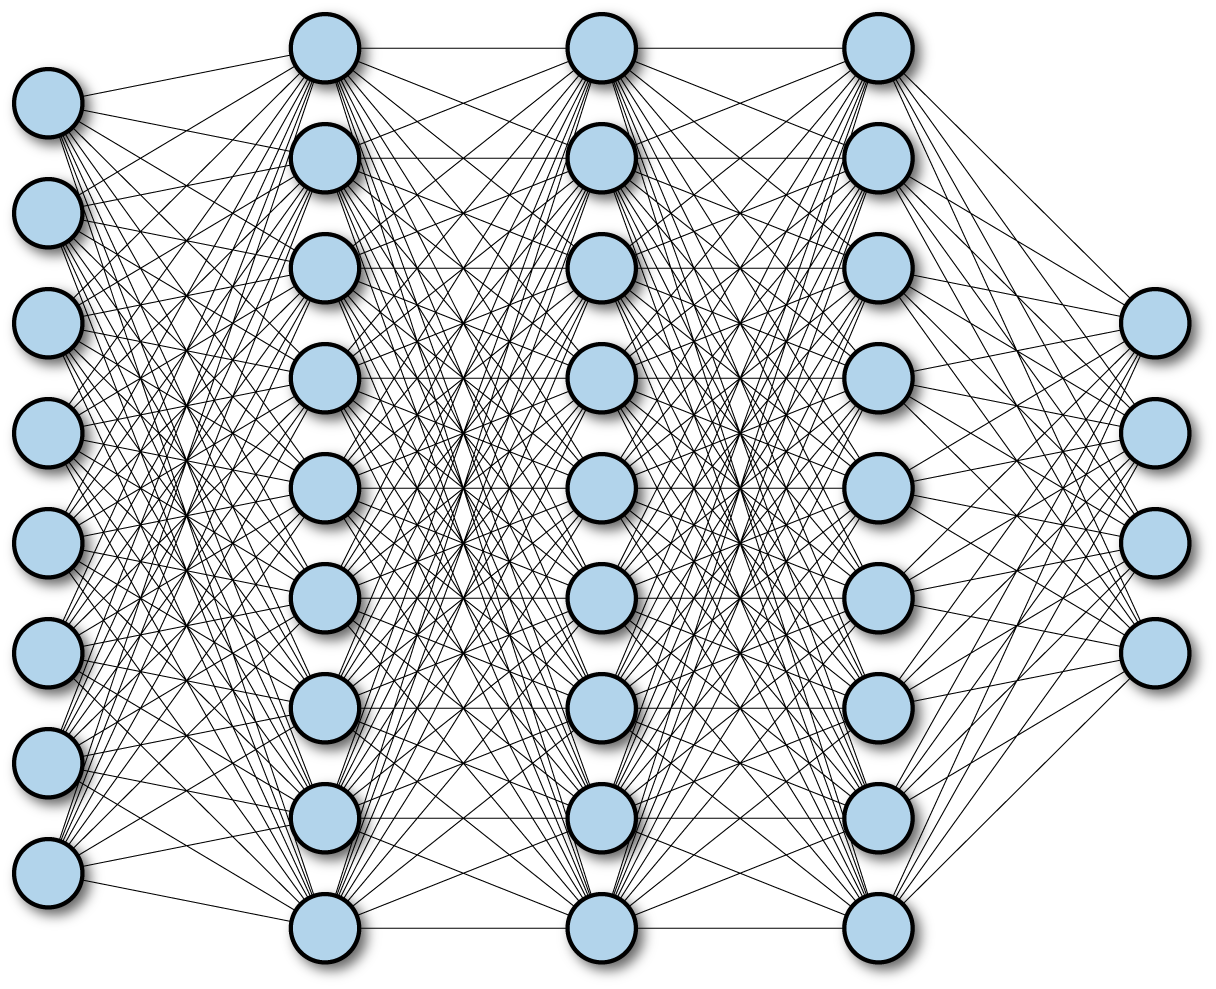
\includegraphics[scale=0.7]{img/fnn_1.png}
\end{center}

% Throughout this task, let $\vx\in\bb{R}^n$ be the input vector and
% $\vy\in\bb{R}^m$ an output vector of such a fully-connected neural network.

\begin{enumerate}[label=(\alph*)]
    \item How many units should we have in the input layer? And in the output
          layer?
    \item What is the difference between the values in nodes and those in edges?
    \item What is the \emph{general} operation performed by each unit (node) in
          the network? What is the input to this operation? Give a formal
          expression for it.
    \item What is the main difference between different types of artificial
          neurons? Give two examples of different types of neurons.
    \item Denote by $\mX\in\bb{R}^{N\times d}$ the input matrix constructed by
          stacking $N$ input vectors $\vx_i\in\bb{R}^d$ as rows. Similarly,
          denote by $\mH_1$ the matrix that contains the corresponding
          representations computed by the first hidden layer, which has $p$
          units. What is the size of $\mH_1$? Give a formal expression for the
          operation that results in $\mH_1$ given input $\mX$.
\end{enumerate}

\section{Backpropagation}

This task is based on a previous task written by Goran Glavas. \\

With backpropagation, we can get gradient information that is useful to update
the parameters of a multi-layer neural network during training.
We start by computing the relevant gradients of the output layer and then
continue backwards by computing the gradients of previous layers based on the
gradients we computed before.

\begin{enumerate}[label=(\alph*)]
    \item What are the \emph{relevant gradients} we care about during training?
    \item The update rules of gradient-based optimizers require that we compute
          gradients of the functions we are optimizing. For example, when
          backpropagating through a layer with sigmoid activations, we will need
          the gradient of the sigmoid function. Show that this gradient is given
          by:
          \begin{align*}
              \sigma(x)' & = \sigma(x) \cdot (1 - \sigma(x)), \text{where } \sigma(x) = \frac{1}{1 + e^{-x}}
          \end{align*}
    \item You are given the toy feed-forward neural network shown in the figure
          below. 
          This network is used to predict one of two classes given three numeric
          input features: $x_1$, $x_2$, and $x_3$. 
          The network has one hidden layer and one output layer, each consisting 
          of two neurons. 
          The activation function on both layers is the sigmoid function.
          \begin{center}
              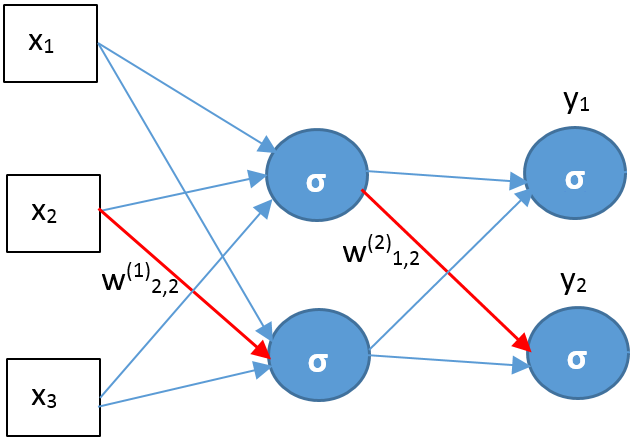
\includegraphics[scale=0.4]{img/backprop_2.png}
          \end{center}
          \begin{enumerate}[label=(\roman*)]
              \item Derive the update rule for the weights marked in red in the
                    image, i.e., for $w^{(1)}_{2,2}$ and $w^{(2)}_{1,2}$.
                    Assume you are training your model with the following square 
                    error loss:
                    \begin{align*}
                        L & = -\frac{1}{2}\frac{1}{N}\sum_{e=1}^{N} \sum_{l=1}^{M} (t_{e,l}-y_{e,l})^2.
                    \end{align*}
                    where $N$ is size of the training set, $M$ is number of 
                    labels, $t_{e,l}$ the target label $l$ of example $e$ and 
                    $y_{e,l}$ the corresponding prediction made by the model.
                    Note that in this toy setting, $M = N = 2$.
                    Using square error loss for a classification task is not a
                    common setting, but it is useful for us to construct a 
                    simple example to study backpropagation.
              \item You are given the toy dataset consisting of the following 
                    two training examples: $([-1, 0, 2], [0, 1])$ and
                    $([2, 1, 1], [1, 0])$.
                    These examples are of the form $(\vx, \vy)$, where $\vx$
                    is input features, and $\vy$ is corresponding label.
                    Assuming that all weights are initialized to $w = 1$, carry 
                    out one update iteration for denoted weights $w^{(1)}_{2,2}$ 
                    and $w^{(2)}_{1,2}$, using the two training examples for 
                    supervision.
                    Use learning rate $\psi = 1$ and the square error 
                    loss given above.
          \end{enumerate}
\end{enumerate}

\section{Skip-Gram Basics}

This task is based on a previous task written by Goran Glavas. \\

Consider the sentence
\begin{align*}
    \textit{The quick brown fox jumped over the lazy dog}, \\
    c_1 \hspace{0.60cm}
    c_2 \hspace{0.60cm}
    w \hspace{0.60cm}
    c_3 \hspace{0.80cm}
    c_4 \hspace{2.35cm}
\end{align*}
where $w$ marks the \emph{center word} and $c_i$ the \emph{context words}.
In this example, we have a \emph{context window} of size $2$, meaning we use the
2 previous and 2 subsequent words around $w$ as context.

In the lecture, we saw how examples for the skip-gram model are constructed and
used to learn a logistic regression model for the task of predicting whether two
given words are in the same context,
\href{https://arxiv.org/pdf/1310.4546.pdf}{\underline{as done by the authors of skip-gram}}.
Formally, they used the following binary classification task to learn word
embeddings: $p(\text{True}|w,c) = \sigma{(l_{w,c})}$ and
$p(\text{False}|w,c) = 1 - p(\text{True}|w,c)$, where $l_{w,c}$ is the logit
score (i.e.\ unnormalized prediction) produced by a logistic regression model
given words $w$ and $c$.
Given this task, sentence and context window, some positive examples of the
form $(\text{source word}, \text{target word})$ would be
$(\textit{fox, quick})$, $(\textit{fox, brown})$, etc.

However, in their
\href{https://arxiv.org/pdf/1301.3781.pdf}{\underline{original work}} on the
skip-gram approach, the authors learned word embeddings using a different task:
predicting context word $c_j$ given center word $w_i$ in position $i$ of a given
sequence of words.
We refer to this task as the \emph{original task} throughout this exercise.

\begin{enumerate}[label=(\alph*)]
    \item How many classes are there in the original task proposed for
          skip-gram? And how could we compute probabilities for each class given
          logit scores from some classifier? Give a formal expression for this
          original task, including the way probabilities are computed from
          logits.
    \item Generate all positive training examples for the original skip-gram
          task using the given sentence above as the entire training set.
          Use a window size of 2.
    \item How is the skip-gram model parameterized? What is the role of each
          parameter?
          Assume your vocabulary consists of 101.425 words and you want to learn
          word representations of 300 dimensions each.
          What is the number of parameters in the skip-gram approach in this
          setting?
    \item Assume that word \textit{Frodo} is the 79th word in your
          vocabulary.
          How do we obtain a single (final) representation of the word
          \textit{Frodo} after our model has finished training?
          What decision do we need to make to obtain such a final
          representation?
\end{enumerate}

\section{Skip-Gram Training}

% ATTENTION! Why give logit scores l here? Do we use than anywhere?!

This task is based on a previous task written by Goran Glavas. \\

We now focus on how to train models using the skip-gram approach.
Assume throughout that we use dot products to compute logit scores, i.e.
$l_{w_i,c_j} = \vw_i^T\vw'_j$, and that we use the softmax function to obtain
probabilities from logit scores

\begin{enumerate}[label=(\alph*)]
    \item To train a skip-gram model, we find the parameters $\vtheta$, i.e.
          word embedings, that maximize the likelihood of our training data,
          i.e.\ we perform MLE.
          Given text corpus $T$, give the expression for the dataset likelihood
          $L(\vtheta|T)$ as determined by a skip-gram model with a context
          window of size $L$.
          Give the corresponding negative log-likelihood expression under the
          empirical risk minimization framework.
          As in the lecture, assume independence between words and between 
          training examples (i.i.d. assumption).
    \item Recall that computing the negative log-likelihood is equivalent to
          using cross-entropy loss.
          Consider the following toy vocabulary
          V=\{\textit{Daenerys}, \textit{Frodo}, \textit{ring}, \textit{dragon}, \textit{Picard}, \textit{ship}\}.
          Assume you are training a skip-gram model over a large corpus $T$ with
          this vocabulary, and that the current values of the parameters of your
          model are the following:
          \[
              \mathbf{W}=
              \begin{bmatrix}
                  0.54 & 0.25 & 0.07 \\
                  0.91 & 0.74 & 0.27 \\
                  0.58 & 0.00 & 0.05 \\
                  0.16 & 0.77 & 0.31 \\
                  0.10 & 0.54 & 0.32 \\
                  0.59 & 0.99 & 0.06
              \end{bmatrix},
              \mathbf{W'}=
              \begin{bmatrix}
                  0.19 & 0.64 & 0.98 \\
                  0.17 & 0.42 & 0.47 \\
                  0.55 & 0.24 & 0.92 \\
                  0.89 & 0.58 & 0.13 \\
                  0.31 & 0.73 & 0.48 \\
                  0.49 & 0.20 & 0.54
              \end{bmatrix}
          \]
          Compute the value of the cross-entropy loss corresponding to the
          single training instance (\textit{Frodo} (source word),
          \textit{ring} (target word)) when used as positive example.
    \item Assume we train using stochastic gradient-descent, i.e. we update our
          relevant parameters during training after computing the loss for a
          single positive example as done in (b).
          Which parameters are updated after every single example? Why?
\end{enumerate}

\section{Word Embeddings as Matrix Factorization}

As discussed in Task 1, we obtain the final representation of a given word from
its corresponding representations in $\mW$ and $\mW'$.
Let us now consider the perspective that $\mW$ and $\mW'$ are factors of another
matrix $\mM$, i.e.\ $\mM = \mW\mW'^T$.
If we can derive some meaning for $\mM$, we may be able to interpret what we are
learning to factorize with the skip-gram approach.

As in the lecture, we now take the perspective of skip-gram as the binary
classification task $p(\text{True}|w,c) = \sigma(\vw_w^t\vw_c)$, where $w$ is a
source word, $c$ a target (context) word, and $\vw_w,\vw_c$ their corresponding
word representations.
Note that in this setting, entry $m_{ij}$ in $\mM$ is given by $\vw_i^T\vw_j$.

\begin{enumerate}[label=(\alph*)]
    \item We saw in the lecture that the skip-gram training objective for
          \emph{a single training example} $(w,c)$ using the cross-entropy loss
          is the following:
          \begin{align}\label{eq:basic_objective}
              L(w,c) = \log \sigma(\vw_w^t\vw_c) + \sum_{i=1}^k \log(-\vw_w^t\vw_i),
          \end{align}
          where $k$ are the number of negative examples sampled per positive
          tuple $(w,c)$ in the training set (we omit the negation of the loss
          for brevity).
          Rewrite Equation~\ref{eq:basic_objective} so that it explicitly shows
          the \emph{sampling} of negatives.
          To this end, use the
          \href{https://en.wikipedia.org/wiki/Expected_value}{\underline{expectation}}
          operator and assume negative examples $\vw_i$ are drawn from the
          uniform distribution $P$ over vocabulary $V$.
          That is, the probability of using word $c$ to construct a negative is
          $\frac{\#(c)}{|V|}$, where $\#(c)$ is the number of times word $c$
          appears in the training corpus.
    \item Generalize your training objective derived in the previous question to
          include all training examples $(w,c)$, i.e.\ the overall training
          objective $L$ using the entire corpus.
    \item During training, we optimize the objective $L$. To see what this
          optimization process tells us about $m_{wc}$, show that the optimal
          value for $\vw_w^t\vw_c$ is given by the following expression:
          \begin{align}\label{eq:pmi_equality}
              \vw_w^t\vw_c = \ln\left(\frac{\#(w,c) |V|}{\#(w) \#(c)}\right) - \ln k
          \end{align}
          To get there, derive an optimal value for $\vw_w^t\vw_c$ by computing
          the gradient of $L$ w.r.t \emph{a single training example} $(w,c)$,
          setting it to zero, and deriving a value for $\vw_w^t\vw_c$. \\
          \textbf{Hint:} only two terms in $L$ are relevant for this gradient
          computation.
\end{enumerate}

\end{document}
